\documentclass[journal,12pt,twocolumn]{IEEEtran}
\makeatletter
\@addtoreset{figure}{problem}
\makeatother
\usepackage{setspace}
\usepackage{gensymb}
\usepackage{xcolor}
\usepackage{caption}
%\usepackage{multirow}
%\usepackage{multicolumn}
%\usepackage{subcaption}
%\doublespacing
\singlespacing
\usepackage{amsmath}
\usepackage{multicol}
\usepackage{enumerate}
\usepackage{amssymb}
\usepackage{graphicx}
\usepackage{newfloat}
%\usepackage{syntax}
\usepackage{listings}
\usepackage{color}
\usepackage{tikz}
\usetikzlibrary{shapes,arrows}



%\usepackage{graphicx}
%\usepackage{amssymb}
%\usepackage{relsize}
%\usepackage[cmex10]{amsmath}
%\usepackage{mathtools}
%\usepackage{amsthm}
%\interdisplaylinepenalty=2500
%\savesymbol{iint}
%\usepackage{txfonts}
%\restoresymbol{TXF}{iint}
%\usepackage{wasysym}
\usepackage{amsthm}
\usepackage{mathrsfs}
\usepackage{txfonts}
\usepackage{stfloats}
\usepackage{cite}
\usepackage{cases}
\usepackage{mathtools}
\usepackage{caption}
\usepackage{enumerate}	
\usepackage{enumitem}
\usepackage{amsmath}
%\usepackage{xtab}
\usepackage{longtable}
\usepackage{multirow}
%\usepackage{algorithm}
%\usepackage{algpseudocode}
\usepackage{enumitem}
\usepackage{mathtools}
%\usepackage{iithtlc}
%\usepackage[framemethod=tikz]{mdframed}
\usepackage{listings}
\usepackage{listings}
    %\usepackage[latin1]{inputenc}                                 %%
    \usepackage{color}                                            %%
    \usepackage{array}                                            %%
    \usepackage{longtable}                                        %%
    \usepackage{calc}                                             %%
    \usepackage{multirow}                                         %%
    \usepackage{hhline}                                           %%
    \usepackage{ifthen}                                           %%
  %optionally (for landscape tables embedded in another document): %%
    \usepackage{lscape}     



%\usepackage{stmaryrd}


%\usepackage{wasysym}
%\newcounter{MYtempeqncnt}
\DeclareMathOperator*{\Res}{Res}
%\renewcommand{\baselinestretch}{2}
\renewcommand\thesection{\arabic{section}}
\renewcommand\thesubsection{\thesection.\arabic{subsection}}
\renewcommand\thesubsubsection{\thesubsection.\arabic{subsubsection}}

\renewcommand\thesectiondis{\arabic{section}}
\renewcommand\thesubsectiondis{\thesectiondis.\arabic{subsection}}
\renewcommand\thesubsubsectiondis{\thesubsectiondis.\arabic{subsubsection}}

% correct bad hyphenation here
\hyphenation{op-tical net-works semi-conduc-tor}

%\lstset{
%language=C,
%frame=single, 
%breaklines=true
%}

%\lstset{
	%%basicstyle=\small\ttfamily\bfseries,
	%%numberstyle=\small\ttfamily,
	%language=Octave,
	%backgroundcolor=\color{white},
	%%frame=single,
	%%keywordstyle=\bfseries,
	%%breaklines=true,
	%%showstringspaces=false,
	%%xleftmargin=-10mm,
	%%aboveskip=-1mm,
	%%belowskip=0mm
%}

%\surroundwithmdframed[width=\columnwidth]{lstlisting}
\def\inputGnumericTable{}                                 %%
\lstset{
language=C,
frame=single, 
breaklines=true
}
 

\begin{document}
%
\tikzstyle{block} = [rectangle, draw,
    text width=3em, text centered, minimum height=3em]
\tikzstyle{sum} = [draw, circle, node distance=3cm]
\tikzstyle{input} = [coordinate]
\tikzstyle{output} = [coordinate]
\tikzstyle{pinstyle} = [pin edge={to-,thin,black}]

\theoremstyle{definition}
\newtheorem{theorem}{Theorem}[section]
\newtheorem{problem}{Problem}
\newtheorem{proposition}{Proposition}[section]
\newtheorem{lemma}{Lemma}[section]
\newtheorem{corollary}[theorem]{Corollary}
\newtheorem{example}{Example}[section]
\newtheorem{definition}{Definition}[section]
%\newtheorem{algorithm}{Algorithm}[section]
%\newtheorem{cor}{Corollary}
\newcommand{\BEQA}{\begin{eqnarray}}
\newcommand{\EEQA}{\end{eqnarray}}
\newcommand{\define}{\stackrel{\triangle}{=}}

\bibliographystyle{IEEEtran}
%\bibliographystyle{ieeetr}

\providecommand{\nCr}[2]{\,^{#1}C_{#2}} % nCr
\providecommand{\nPr}[2]{\,^{#1}P_{#2}} % nPr
\providecommand{\mbf}{\mathbf}
\providecommand{\pr}[1]{\ensuremath{\Pr\left(#1\right)}}
\providecommand{\qfunc}[1]{\ensuremath{Q\left(#1\right)}}
\providecommand{\sbrak}[1]{\ensuremath{{}\left[#1\right]}}
\providecommand{\lsbrak}[1]{\ensuremath{{}\left[#1\right.}}
\providecommand{\rsbrak}[1]{\ensuremath{{}\left.#1\right]}}
\providecommand{\brak}[1]{\ensuremath{\left(#1\right)}}
\providecommand{\lbrak}[1]{\ensuremath{\left(#1\right.}}
\providecommand{\rbrak}[1]{\ensuremath{\left.#1\right)}}
\providecommand{\cbrak}[1]{\ensuremath{\left\{#1\right\}}}
\providecommand{\lcbrak}[1]{\ensuremath{\left\{#1\right.}}
\providecommand{\rcbrak}[1]{\ensuremath{\left.#1\right\}}}
\theoremstyle{remark}
\newtheorem{rem}{Remark}
\newcommand{\sgn}{\mathop{\mathrm{sgn}}}
\providecommand{\abs}[1]{\left\vert#1\right\vert}
\providecommand{\res}[1]{\Res\displaylimits_{#1}} 
\providecommand{\norm}[1]{\lVert#1\rVert}
\providecommand{\mtx}[1]{\mathbf{#1}}
\providecommand{\mean}[1]{E\left[ #1 \right]}
\providecommand{\fourier}{\overset{\mathcal{F}}{ \rightleftharpoons}}
%\providecommand{\hilbert}{\overset{\mathcal{H}}{ \rightleftharpoons}}
\providecommand{\system}{\overset{\mathcal{H}}{ \longleftrightarrow}}
	%\newcommand{\solution}[2]{\textbf{Solution:}{#1}}
\newcommand{\solution}{\noindent \textbf{Solution: }}
\providecommand{\dec}[2]{\ensuremath{\overset{#1}{\underset{#2}{\gtrless}}}}
\DeclarePairedDelimiter{\ceil}{\lceil}{\rceil}
%\numberwithin{equation}{subsection}
\numberwithin{equation}{problem}
%\numberwithin{problem}{subsection}
%\numberwithin{definition}{subsection}
\makeatletter
\@addtoreset{figure}{problem}
\makeatother

\let\StandardTheFigure\thefigure
%\renewcommand{\thefigure}{\theproblem.\arabic{figure}}
\renewcommand{\thefigure}{\theproblem}


%\numberwithin{figure}{subsection}

%\numberwithin{equation}{subsection}
%\numberwithin{equation}{section}
\numberwithin{equation}{problem}
%\numberwithin{problem}{subsection}
\numberwithin{problem}{section}
%%\numberwithin{definition}{subsection}
%\makeatletter
%\@addtoreset{figure}{problem}
%\makeatother
\makeatletter
\@addtoreset{table}{problem}
\makeatother

\let\StandardTheFigure\thefigure
\let\StandardTheTable\thetable
%%\renewcommand{\thefigure}{\theproblem.\arabic{figure}}
%\renewcommand{\thefigure}{\theproblem}

%%\numberwithin{figure}{section}

%%\numberwithin{figure}{subsection}



\def\putbox#1#2#3{\makebox[0in][l]{\makebox[#1][l]{}\raisebox{\baselineskip}[0in][0in]{\raisebox{#2}[0in][0in]{#3}}}}
     \def\rightbox#1{\makebox[0in][r]{#1}}
     \def\centbox#1{\makebox[0in]{#1}}
     \def\topbox#1{\raisebox{-\baselineskip}[0in][0in]{#1}}
     \def\midbox#1{\raisebox{-0.5\baselineskip}[0in][0in]{#1}}

\vspace{3cm}

\title{ 
%	\logo{
RLS Adaptive Filter
%	}
}

\author{B Swaroop Reddy and Dr G V V Sharma$^{*}$% <-this % stops a space
	\thanks{*The author is with the Department
		of Electrical Engineering, Indian Institute of Technology, Hyderabad
		502285 India e-mail:  gadepall@iith.ac.in. All content in this manual is released under GNU GPL.  Free and open source.}
	
}	

\maketitle

\tableofcontents
\bigskip

\begin{abstract}
	
	This manual explains about how the Adaptive Recursive Least Squares Algorithm can be used for noise-cancellation in the speech signal and as an Equalizer in a communication system.
	
\end{abstract}

\section{RLS Algorithm}
Consider the following block diagram(Fig.1.0) for the structure of the adaptive LMS filter.
\begin{figure}
\centering
\begin{tikzpicture}[auto, node distance=2cm,>=latex']
    % We start by placing the blocks
     \node [input, name=input] {};
    \node [block, right of=input,node distance=4cm] (a) 
    {Adaptive filter $W(n)$};
    \node [block, below of=a, node distance=3cm] (b) {Adaptive RLS Algorithm};
    \draw [->] (b) -- node[name=u] {$W(n+1)$} (a);
    \node [sum, right of=a,pin={[pinstyle]above:$d(n)$},
            node distance=4cm] (sum) {$+$};
    \node [output, right of=sum] (output) {}; 
    \draw [->] (input) -- node [name=x] {$X(n)$} (a);
    \draw [->] (a) -- node[pos= 0.90]{$-$} node 
      {$y(n)$}  (sum);
    \draw [->] (sum) -- node [name=e] {$e(n)$}(output);
    
    \draw [->] (sum) |- node {$e(n)$} (b) ;
    \draw [->] (x) |- node {} (b);
\end{tikzpicture}
\caption{The Adaptive RLS filter} \label{fig1}
\end{figure}
Where
\begin{itemize}
\item  
\begin{gather}
 X(n)
 =
 %\frac{1}{\det(X)}
  \begin{bmatrix}
   X(n) \\ X(n-1)\\
   X(n-2) \\ $..$ \\ $..$ \\ X(n-M+1)  \end{bmatrix}_{M X 1}
\end{gather}
\item
\begin{gather}
 W(n)
 =
 %\frac{1}{\det(X)}
  \begin{bmatrix}
   w_1(n) \\ w_2(n)\\
   w_3(n) \\ $..$ \\ $..$ \\ w_{n-M+1}(n)  \end{bmatrix}_{M X 1}
\end{gather}
\end{itemize}
\begin{problem}
Write the expression for the error from Fig\ref{fig1}
\label{prob1}
\end{problem} 
\solution
\begin{align*}
e(n)&=d(n) - y(n)\\
&=d(n) - W^{T}(n) X(n)\\
&=d(n) - X^{T}(n)W(n)\\
\end{align*}
\begin{problem}
Write the expression for cost function for adaptive RLS Algorithm. \label{prob2}
\end{problem}
\solution
\begin{align*}
J(n) &= \sum_{i=1}^{n} \beta (n,i) |e(n)|^2
\end{align*}
The weighting factor $\beta (n,i)$ has the property $0<\beta (n,i)\leq 1$ ,   i=1,2,...,n\\
A special form of weighting is Exponential Weighting factor i.e $\beta (n,i)$ = $\lambda ^{n-i}$ ,  i=1,2,...,n\\
Therefore,
\begin{align*}
J(n) &=\sum_{i=1}^{n} \lambda ^{n-i} |e(n)|^2 \\
&=\sum_{i=1}^{n} \lambda ^{n-i}[(d(i) - W^{T}(n)X(i))^{T}(d(i) - W^{T}(n)X(i))]
\end{align*}
\begin{problem}
Write the expressions for the optimal solution from the cost function.
\end{problem}
\solution
\begin{align*}
\frac{\partial J(n)}{\partial W(n)}=0\\
\sum_{i=1}^{n} \lambda ^{n-i}[0 - X(i)d^{T}(i)-X^{T}(i)d(i)+2W(n))X(i)X^{T}(i)]=0\\
[\sum_{i=1}^{n} \lambda ^{n-i}X(i)X^{T}(i)]W(n)=\sum_{i=1}^{n} \lambda ^{n-i}X(i)d^{T}(i)\\
\phi (n) \hat W(n) =z(n)
\end{align*}
\begin{equation}
\hat W(n) =\phi ^{-1} (n) z(n)
\end{equation}
Where 
\begin{itemize}
\item $\hat W(n)$ is the optimal value of the Tap-Weight vector
\item $\phi (n) = \sum_{i=1}^{n} \lambda ^{n-i}X(i)X^{T}(i)$
\item $z(n) = \sum_{i=1}^{n} \lambda ^{n-i}X(i)d^{T}(i)$
\end{itemize}
\begin{align*}
\phi (n) &= \sum_{i=1}^{n-1} \lambda ^{n-i}X(i)X^{T}(i)+X(n)X^{T}(n)\\
&=\lambda \sum_{i=1}^{n-1} \lambda ^{n-i}X(i)X^{T}(i)+X(n)X^{T}(n)
\end{align*}
\begin{equation}
\phi (n)=\lambda \phi (n-1) + X(n)X^{T}(n)
\end{equation}

Where $\phi (n-1)$ is the old value of the correlation matrix and $X(n)X^{T}(n)$ plays a role of a correction term in the updating operation\\
Similarly, 

\begin{equation}
z(n)=\lambda z(n-1) + X(n)X^{T}(n)
\end{equation}
\textbf{Matrix Inversion Lemma:}\\
Let A and B be two positive-definite M X M matrices related by
\begin{align*}
A&=B^{-1}+CD^{-1}C^{T}
\end{align*}
Where D is another positive-definite N X M matrix and C is an M X N matrix, then
\begin{align*}
A^{-1}&=B-BC(D+C^{T}BC)^{-1}C^{T}B
\end{align*}
\begin{problem}
Derive the time update for the  Tap-weight vector for Exponentially weighted RLS adaptive filter.
\end{problem}
\solution
From equation 1.3.2 \\
\begin{align*}
 A&=\phi (n)\\
 B^{-1}&=\lambda \phi(n-1)\\
 C&=X(n)\\
 D&=1\\
\end{align*}
By Applying matrix inversion lemma - \\
\begin{align*}
\phi ^{-1} (n) &= \lambda ^{-1} \phi ^{-1} (n-1) - \\ & \dfrac{\lambda ^{-2}\phi ^{-1} (n-1)X(n)X^{T}(n)\phi ^{-1} (n-1)}{1+\lambda ^{-1}X^{T}(n)\phi ^{-1} (n-1)X(n)}\\
P(n)&=\lambda ^{-1}P(n-1) - \lambda ^{-1} K(n)X^{T}(n)P(n-1)
\end{align*}
Where \\
\begin{equation}
P(n)=\phi ^{-1} (n)
\end{equation} and 
\begin{equation}
K(n) = \dfrac{\lambda ^{-1}P(n-1)X(n)}{1+ \lambda ^{-1}X^{T}(n)P(n-1)X(n)}
\end{equation}
From equation (1.4.2)
\begin{align*}
K(n) &=\lambda ^{-1}P(n-1)X(n)-\lambda ^{-1}K(n)X^{T}(n)P(n-1)X(n)\\
K(n)&=(\lambda ^{-1}P(n-1)-\lambda ^{-1}K(n)X^{T}(n)P(n-1))X(n)
\\
K(n)&=P(n)X(n)
\end{align*}
\begin{equation}
K(n)=\phi ^{-1} (n)X(n)
\end{equation}
From equation (1.3.2)
\begin{align*}
\hat W(n) &=\phi ^{-1}(n)z(n)\\
&=P(n)z(n)\\
&=\lambda P(n)z(n-1) + P(n) X(n) d^{T}(n)\\
&=P(n-1)z(n-1)-K(n)X^{T}(n)P(n-1)z(n-1) \\ &+P(n) X(n) d^{T}(n)\\
&=\phi ^{-1}(n-1)z(n-1)-K(n)X^{T}(n)\phi ^{-1}(n-1)z(n-1) 
\\ & +P(n) X(n) d^{T}(n)\\
&=\hat W(n-1)-K(n)X^{T}(n)\hat W(n-1) +P(n) X(n) d^{T}(n)\\
&=\hat W(n-1)-K(n)X^{T}(n)\hat W(n-1) +K(n)d^{T}(n)\\
&=\hat W(n-1)+K(n)[-X^{T}(n)\hat W(n-1) +d^{T}(n)]\\
&=\hat W(n-1)+K(n)e_{*}^{T}(n)\\
\end{align*}
where\\
\begin{equation}
e_{*}(n) = d(n)-\hat W^{T}(n-1)X^{T}(n) 
\end{equation}
is a priori estimation error and\\
\begin{equation}
e(n) = d(n)-\hat W^{T}(n)X^{T}(n) 
\end{equation}
is a posteriori estimation error.\\ \\
\medskip
\textbf{Summary of the RLS algorithm}
\begin{enumerate}
\item Initialize the algorithm by setting P(0)=$\delta ^{-1} I$,where$\delta$ = small positive constant\\
$\hat W^{T}(0)=0$ 
\item For each instant of time, n=1,2,3,....\\
 compute the following
 \begin{align*}
 K(n) &= \dfrac{\lambda ^{-1}P(n-1)X(n)}{1+ \lambda ^{-1}X^{T}(n)P(n-1)X(n)}\\
e(n) &= d(n)-\hat W^{T}(n-1)X^{T}(n)\\
\hat W(n)&=\hat W(n-1)+K(n)e_{*}^{T}(n)\\
P(n)&=\lambda ^{-1}P(n-1) - \lambda ^{-1} K(n)X^{T}(n)P(n-1)\\
\end{align*}
\end{enumerate}
\section{Adaptive Noise Cancellation}
You will need two data streams: one corresponding to signal plus noise and the other corresponding to noise.\\

Consider the following M-th order FIR adaptive structure for noise cancellation.\\
\begin{figure}
\centering
%\includegraphics[width=\columnwidth]{./figs/figure1.eps}
\begin{tikzpicture}[auto, node distance=2cm,>=latex']
    % We start by placing the blocks
     \node [block, name=signal] {Signal Source};
    \node [sum, right of=signal,node distance=2cm] (sum) {};
    \node [block, below of=signal,node distance=3cm] (noise) 
    {Noise Source};
    \node [sum, right of=noise, node distance=2cm] (sum1){};
    \draw [->] (noise) -- node[below][pos= 0.99]{$+$} node[below] 
      {$X(n)$}  (sum);
    \draw [->] (noise) -- node {$X(n)$} (sum1);
    \node [sum, right of=sum,node distance=4cm] (sum2) 
    {};
    \node [block, right of=sum1,node distance=2cm] 
    (filter) {Adaptive RLS filter};
    \draw [->] (signal) -- node[pos= 0.99]{$+$} node 
      {$S(n)$}  (sum);
    \draw [->] (sum) -- node [pos= 0.99]{$+$} node {$S(n) + 
    X(n) = d(n)$} (sum2);
    \draw [->] (sum1) -- node [name=x] {$X(n)$} (filter);
    \draw [->] (filter) -| node [pos= 0.99]{$-$} 
    node[name=y][below] {$y(n)$} (sum2);
    \node [output, right of=sum2,node distance=2cm] (output) {};
    \draw [->] (sum2) -- node [name=out]{$\hat S(n)$} (output);
   % \draw [-] (out) |- node {$e(n)$} (filter);
    \node [output, above of=x,node distance=1.5cm] (output1) {};
    \node [output, below of=y,node distance=1.5cm] (output2) {};
    \draw [-] (out) |- node {$e(n)$} (output2);
    \draw [-] (output2) -- node {} (filter);
   \path [draw, ->] (filter) -- node [above] {} 
        (output1);
    \end{tikzpicture}
\caption{RLS Noise Cancellation System}
\label{fig:2}
\end{figure}

Assume that $X(n)$ and S(n) are statistically independent.Let $e(n)=S(n)+X(n)-\hat X(n)$.
\begin{problem}
Download the sound file from\\
%http://tlc.iith.ac.in/img/speech/signal_noise.wav and
%http://tlc.iith.ac.in/img/speech/noise.wav\\
The files are for speech plus noise, and only noise. You will notice that you cannot decipher the speech when you play the speech plus noise file; but upon proper implementation of the noise cancellation algorithm you will be able to decipher the speech.\\
\label{prob2.1}
\end{problem}
\begin{problem}
Using the speech samples in Problem \ref{prob2.1} write a python script for the Adaptive noise cancellation using LMS algorithm.\\ \label{prob2.2}
\end{problem}
\solution
	  \lstinputlisting{./RLS_NC_SPEECH.py}
	  
\begin{problem}
The output of the python script in Problem \ref{prob2.2} is the speech signal output\_ signal\_ rls.wav.Listen to the the speech signal. What do you observe?	 
\end{problem} 
\section{Adaptive Equalization}
\textbf{RLS algorithm for channel equalization using training signals:}\\
Consider the following block diagram for the adaptive channel equalizer using training sequences.\\
\begin{center}
\begin{figure}
\centering
%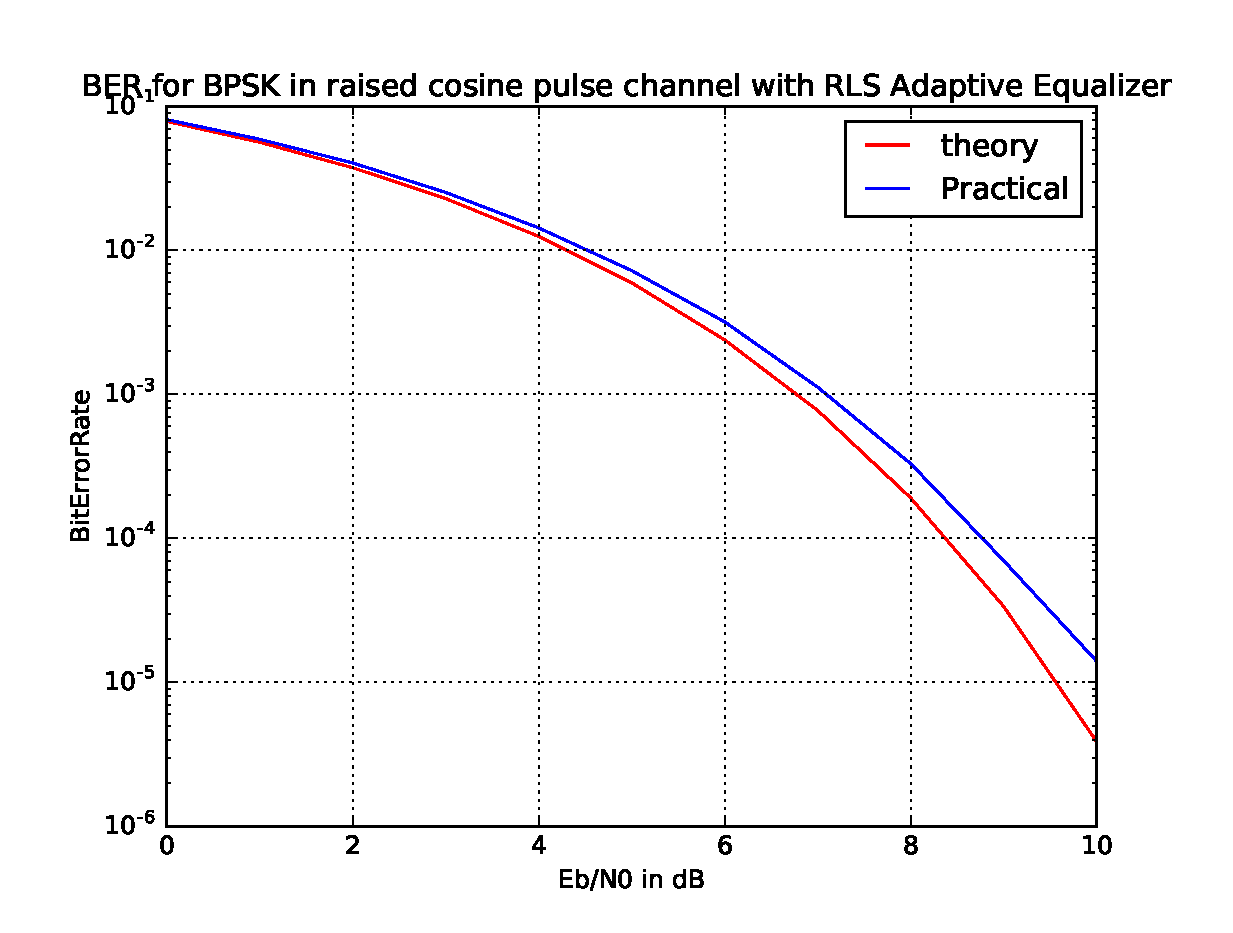
\includegraphics[width=\columnwidth]{SNR_Vs_BER.eps}

\begin{tikzpicture}[auto, node distance=2cm,>=latex']
    % We start by placing the blocks
     \node [block, name=binary] {Binary Symb Generator};
    \node [block, right of=binary,node distance=2cm] (channel) {Channel $h(n)$};
    \draw [->] (binary) -- node[below][name=b] {$b_n$} (channel);
    \node [block, above of=channel,node distance=3cm] (delay) {Delay};
    \node [sum, right of=channel, node distance=1.5cm] (sum){$\sum$};
    \draw [->] (channel) -- node {}  (sum);
    \draw [->] (b) |- node {} (delay);
    \node [block, right of=sum,node distance=1.5cm] (filter) 
    {Adaptive RLS filter};
    \node [sum, right of=filter,node distance=1.5cm] 
    (sum1) {$\sum$};
    \draw [->] (sum) --  node[name=x] {$x(n)$}  (filter);
    \node [block, below of=sum,node distance=3cm] (noise) {AWGN Generator};
    
    \draw [->] (noise) -- node [pos= 0.95]{$+$} node {$v(n)
    $} (sum);
    \draw [->] (delay) -| node [name=a] {$b(n-7))$} (sum1);
    \draw [->] (filter) -- node [pos= 0.99]{$-$} node[name=y] {} (sum1);
    \node [output, below of=x,node distance=2cm] (output1) {};
    \draw [-] (sum1) |- node [name=e]{$e(n)$} (output1);
    \draw [-] (output1) -- node {} (filter);
    
    \node [output, above of=y,node distance=2cm] (output2) {};
    \draw [->] (filter) -- node {} (output2);
    \node [block, right of=sum1,node distance=1.5cm] (decision) {Hard Threshold};
  \node [output, below of=decision,node distance=1cm] (output3) {};
   \draw [-] (y)|- node {} (output3);
   \draw [->] (output3)-- node {} (decision);
   \node [output, right of=decision,node distance=1.5cm] (output) {};
  
   \draw [->] (decision)-- node {$\hat b_n$} (output);
    
\end{tikzpicture}
\caption{RLS Equalization System}
\label{fig:f3}
\end{figure}
\end{center}


\bigskip
In the above we are assuming that the transmitted symbols are binary (bpsk) with zero mean $b_n=\pm 1$. These are passed through a channel with impulse response\\
\medskip
$h(n)=\begin{cases}
\frac{1}{2}[1+cos(\frac{2\pi}{F}{(n-2)})]& n=1,2,3\\
0 & otherwise
\end{cases}$\\
\medskip
and corrupted by additive white Gaussian noise (AWGN) with zero mean and variance $\sigma^2$. The delayed symbols that are fed at the output of the adaptive filter act as training signals.The channel impulse response is an 3-point FIR filter with a raised cosine type of structure.Parameter F controls the eigen value spread of $R=E[X(n)X^T(n)$.\\
\medskip
Note:\\ 
$$x(n)=\quad\sum_{k=1}^{3}h(k)b_{n-k}+v(n)$$\\
\medskip
You will need two random number generators; one for the symbols b n and the other for the AWGN.For AWGN assume $\sigma^2=0.001.$ For $b_n$ use a binary random number generator where 1 and -1 are generated with equal probability. You could do this by using a uniform random number generator, uniform over [−0.5, 0.5]. Whenever you get a negative number, set it to -1 and whenever you get a positive number set it to +1.
\medskip
\begin{problem}
At the output of the adaptive filter have a hard threshold unit to classify the output as 1 or -1. This is done since we know that the transmitted symbols were 1 or -1. Now write a python script to compute the percentage bits that are in error at convergence (this will give you the bit error rate (BER)) with different SNRs. Plot the SNR Vs BER curve.
\end{problem}
\solution
	  \lstinputlisting{./RLS_Equalizer.py}
\begin{center}
\begin{figure}
\centering
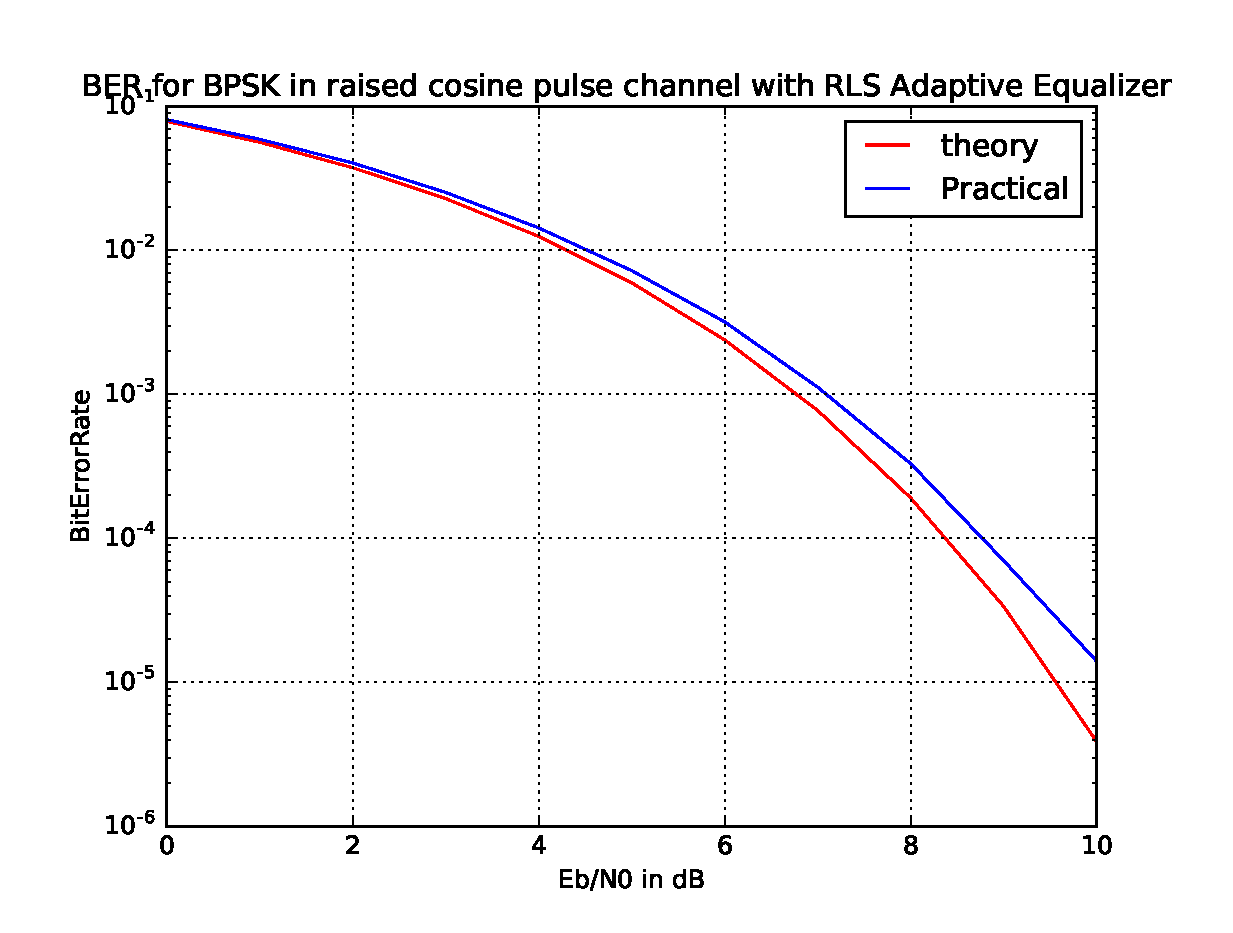
\includegraphics[width=\columnwidth]{SNR_Vs_BER.eps}
\caption{}
\label{fig:f3}
\end{figure}
\end{center}

\begin{problem}

The channel is no longer as given by the cosine function. But, now let the channel be modeled by an FIR filter of length 10, and each FIR coefficient be of unit magnitude. Repeat the above channel equalization problem for the equalizer under a narrow band channel.Plot the bit error rate.
\end{problem}
\begin{problem}
The data symbols are not binary (BPSK) but are QPSK. You can generalize the method used for generating BPSK to a method for generating QPSK. Plot the bit error rate. Do this for both the cases: (a) the FIR channel specified above, and (b) any other narrow band channel of your choice.
\end{problem}

\end{document}